%Contributer: Kendal Sandridge, Colin Tan
{\parindent0pt
\section{Spectral Clustering}

As of late Spectral Clustering has become exceedingly popular due to the quality of its clusters compared to other clustering algorithms.   It is possible to turn clustering into a graph problem, then solve it by figuring out the cut that splits our graph into the groups with high intracluster weights. One of the benefits of this formulation is that the data can be in any space, not just euclidean, and we can still perform clustering. \\

We can formulate the problem of spectral clustering with well defined inputs and outputs

\textbf{Input:} \\
- $x_1,...,x_n$ data points\\
- $w_{ij}$ similarity between points $x_i, x_j$ \\

\textbf{Goal}\\
- MINIMIZE intercluster weights\\
- MAXIMIZE intracluster weights\\



We first introduce the notion of a similarity graph. We can construct a similarity graph from a set of points $S$, and a similarity function that returns a value $s_{ij}$, the similarity from points $i, j \in S$. In this way we construct a graph $G = (V,E)$ where $V = S$ and $(i,j) \in E$ if $s_{ij} > 0$.  The weights of each edge in the weights matrix would be $s_{ij}$ if $s_{ij}$ is positive and 0 otherwise. There are actually many ways of constructing the weight matrix $W$ of $G$. A few are listed below:\\

\textbf{Methods of creating W}
\begin{itemize}
	\item k-NN graph
	\item $\epsilon$-neighbor graph
	\item Gaussian kernel $w_{ij} = exp(\dfrac{-\lVert x_i - x_j\rVert ^2}{2 \sigma ^2})$
\end{itemize}

A few facts about the weights matrix is that if $w{ij} = 1 \Longleftrightarrow (i,j) \in E$, then $W$ is the usual adjacency matrix. Also $W$ is symmetric. \\


We can define the degree of the a vertex, $v \in V$ to be:
\begin{center}
	\[ d_i := \sum_{j \in V} w_{ij}\]
\end{center}

From this we can also define a degree matrix, $D$:
\begin{center}
	$D = diag(d_i, ..., d_n)$	
\end{center}

\textbf{Useful Notation}\\
It is also helpful to define an edge function $E(S,T)$:
\begin{center}
	Given that $S, T \subset V$ $ E(S,T) := \{(i,j) \in E : i \in S, j \in T\}$\\
\end{center}

We denote the compliment of a set of vertices, $\bar{S}$ as:
\begin{center}
	$\bar{S} := S \setminus V$
\end{center}

For shorthand we denote:
\begin{center}
	$\delta S = E(S, \bar{S})$
\end{center}

It is also important to have a notion of size for a set of vertices. The first is simply the cardinality of the set. The second is the volume of the set defined below.
\textbf{Measures of Size} $S \subset V$: \\
\begin{center}
	\item \[vol(S) := \sum_{i \in S} d_i = \sum_{\substack{i\in S \\
			j\in V}} w_{ij} = weight(E(S, V))\]
\end{center}


\textbf{The MINCUT Problem}\\
\[  \underset{{\emptyset \varsubsetneq S \varsubsetneq V}}{\mathrm{min}}  weight(E(S,\bar{S})) = weight(\delta S) \]\\

\textbf{Fact} \textit{(Stoer-Wagner, 1995)}. There is an efficient algorithm that solves MINCUT.\\
	
	Question: Is this good for clustering?\\
	A: No. We can try to "balance" the size of each partition but turns out the problem become NP-hard \textit{(Wagner \& Wagner 19)}\\
	
	\subsection{Spectral Graph Theory}
	At its heart, the graph Laplacian, L.
	
	\textbf{Review of Laplacian}
	$G = (V,E)$
	Dictionary between discrete calculus \& vector calculus:

	\begin{multicols}{2}
		\textbf{Discrete Calculus}\\
		\begin{itemize}
		\item $V$ is sparse  
		\item $\mathbb R^V$ is space of vertex functions\\
			 inner product space: $\langle f,g\rangle_v := \sum_{i\in V} f(i)g(i)$
		
		\item $\mathbb R^E$ is space of alternating vertex functions
			 \[X([i,j] = -X([j,i]) \textrm{for} (i,j) \in E \]
			inner product space: \[\langle X,Y\rangle_E := \sum_{e \in E} w_e X(e) Y(e) \]
		\item $d$ the derivative operator
		\[d: \mathbb R^V \rightarrow \mathbb R^E\]
		\[ df([i,j]) = f(j)-f(i)\]
		\item Dirichlet energy, measure of smoothness
		\[\mathcal E(f) := \langle df,df\rangle_E = \sum_{\substack{(i,j)\\
				{i < j}}} w_{ij} (f(i)-f(j))^2\]\\
		\end{itemize}
		\columnbreak
		\textbf{Vector Calculus}
		\begin{itemize}
			\item $\mathcal M$ is sparse
			\item $\mathcal C^{\infty}(\mathcal M; \mathbb R)$ space of functions 
			\item $\nabla$ gradient operator
			\item $\mathcal E(f) := \int_{\mathcal M} \lVert \nabla f \rVert ^2$
		\end{itemize}
	\end{multicols}
	Recall the adjoint.\\
	\begin{center}
		if $T: A \rightarrow B$ map of finite-dimension inner product spaces, then\\
		$\exists! T*: B \rightarrow A$ s.t. $\forall a \in A, b \in B, <a, Ta>_B = \langle T*b, a\rangle_A$
	\end{center}
	
	The Laplacian $L$ defined so that:
	\begin{center}
		$\langle df, df\rangle_E = \langle f,Lf\rangle_V$
	\end{center}
	
	Why consider L? In order to form an optimization problem!
	e.g. 
	\begin{center}
		$min \langle df, df\rangle_E $ \indent Lagrange Multipliers $\rightarrow Lf = \lambda f$\\
		s.t. \[ \lVert f \rVert ^2 = 1 \]
	\end{center}
	
	\textbf{Properties of Laplacian}
	\begin{enumerate}
		\item $L = D - W$
		\item $\mathbbm{1} \in ker(L)$
		\item $L \in Sym(\mathbbm R^{n\times n})$
		\item let $A \subset V$. $\mathbbm 1_A^T L \mathbbm 1_A = \sum_{(i,j) \in E} w_{ij} (\mathbbm  1_A(i - \mathbbm 1_A(j)) )^2 = weight(E(A, \bar{A})) $
	\end{enumerate}
	
	\subsection{Review of Spectral Theory: Geometric \& Variational Characterization of Eigenvalues}
	
	\begin{definition}
		Let $M \in \mathbb R^{n \times n}$. An eigenvector $v \in \mathbb R^n$ satisfies $v \neq 0, \exists\lambda \in \mathbb R $ s.t. $Mv = \lambda v$
		The eigenvalues of this matrix form its spectrum.
	\end{definition}
	
	\begin{theorem}[Spectral Theorem for Symmetric Matrices]
		
		Geometric characterization
		
		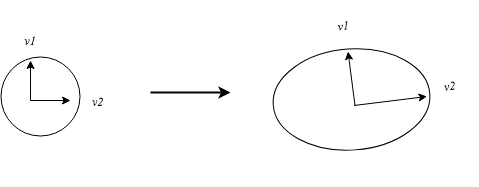
\includegraphics[width=0.8\textwidth]{chapter_3/files/spec_clust_diag.png}
	\end{theorem}
	
	\begin{definition}
		Let $v \neq 0 $ in $\mathbb R^n, \mathcal M \in Sym(\mathbb R{n \times n})$
		Rayleigh Quotient
		$\mathcal R(v) = \dfrac{v^T M v}{v^Tv}$
		
		Notice: $\mathcal R(\alpha v) = Rank(v) \forall \alpha \in \mathbb R \ \{0\}$, can assume $v \in S^{n-1}$
	\end{definition}
	
	
	\begin{theorem}[Variational Characterization]
		Let $M \in Sym(\mathbb R^{n\times n})$\\
		$\lambda_1 \leq ... \leq \lambda_n$ eigenvalues of $M$ \\
		$\lambda_1 = \min_{v \in S^{n-1}} Rank (v)$\\
		$\vdots$ \\
		$\lambda_i = \min_{\substack{ v \in S^{n-1}\\
				v \perp < v_1 ... v_{i-1} >}} Rank (v)$ \\
		$\vdots$ \\
		$\lambda_m = \max_{v \in S^{n-1}} Rank (v)$
	\end{theorem}
	
	\subsection{Spectral Clustering Algorithm}
	
	After introducing the graph Laplacian, we present the spectral clustering algorithm that projects data onto lower dimension space. The algorithm needs predefined number of clusters, and the similarity matrix.
	
	\textbf{Input:} $S$: $n\times n$ similarity matrix (on $n$ data points), $k$: number of clusters.
	
	\textbf{Output:} the partition of $n$ data points returned by $k$-means as the clustering.
	
	\begin{algorithm}
		\caption{Spectral Clustering}
		\begin{algorithmic}
			\STATE Compute the degree matrix $D$ and adjacency matrix $W$ from the weighted graph induced by $S$.
			\STATE Compute the graph Laplacian $L = D - W$.
			\STATE Compute the bottom $k$ eigenvectors $u_1,\ldots,u_k$ of the generalized eigensystem $\mathbf{Lu} = \lambda \mathbf{Du}$.
			\STATE Let $U$ be the $n \times k$ matrix containing vectors $u_1,\ldots,u_k$ as columns.
			\STATE Let $y_i$ be the $i$-th row of $U$; it corresponds to the $k$ dimensional representation of the datapoint $x_i$.
			\STATE Cluster points $y_1,\ldots,y_n$ into $k$ clusters via a centroid-based algorithm like $k$-means.
		\end{algorithmic}
	\end{algorithm}
	
	One can calculate similarity from distance using a drop off function $e^{-\mathrm{dist}^2/\sigma^2}$.
	
	\subsection{Planted Partitions Model}
	
	The need to calculate the eigenvector of the $n\times n$ Laplacian puts the spectral clustering algorithm at $O(n^3)$ runtime. There is an $O(n \log^3 n + m \log n)$ algorithm for Planted Partitions Model problem, as described in \cite{bsh10}.
	
	The Planted Partitions Model problem: for a $(p,q)$-clusetered graph $G(V,E)$, vertices are divided into disjoint clusters $C_1, \ldots, C_t$. Edges between members within clusters are included with probability $p$, and between members across clusters with probability $q$.
	
	Note that $C(v)$ is the cluster containing vertex $v$, and $N(G,v)$ are the neighbors of $v$.
	
	For $p \geq 1/2$, the following Subsquare algorithm described in \cite{bsh10} finds partitions $U_1, \ldots, U_s$ with probability $1-1/\mathrm{poly}(n)$ that for each input cluster $C_i$ of size $\Omega(\max \{qn, \log n \})$, contains a cluster $U_j$ such that $C_i=U_j$. The algorithm takes three parameters, $c_0$, $c_1$, and $\delta$.
	
	\begin{algorithm}
		\caption{Planted Partition Clustering}
		\begin{algorithmic}
			\STATE Randomly order the the vertices with a bijection $\pi : V \rightarrow \{1, \ldots, n\}$.
			\FORALL{$v$, for two passes}
			\STATE If $|N(G,v)|<c_0 \log(n/\delta)$, assign $v$ to its own cluster and continue to the next $v$.
			\STATE Let $R_{temp}$ be the neighbors of $v$ that have been clustered.
			\STATE For each element of $R_{temp}$, include it in $R$ with probability $\min \left\{\frac{c_{0} \log (n / \delta)}{\left|R_{t e m p}\right|}, 1\right\}$.
			\STATE For each element of $N(G,v)$, include it in $S$ with probability $\frac{c_{0} \log (n / \delta)}{|N(G, v)|}$. Similarly for each element of $N(G,w)$, include it in $S_w$ with probability $\frac{c_{0} \log (n / \delta)}{|N(G, w)|}$.
			\STATE Initialize a candidate cluster set $\mathcal{D}$ for $v$ to empty set.
			\FORALL{$w \in R$}
				\IF{$|S \cap N(G, w)| \geq c_{1} \log (n / \delta)$, $|N(G, w)| \geq c_{0} \log (n / \delta)$ and $\left|S_{w} \cap N(G, v)\right| \geq c_{1} \log (n / \delta)$}
					\STATE add $w$'s cluster $\hat{C}(w)$ to $\mathcal{D}$.
				\ENDIF
			\ENDFOR
			\ENDFOR
			\STATE If $\mathcal{D}$ is not empty, set $\hat{C}(v)=\hat{C}\left(\operatorname{argmin}_{w^{\prime} \in \cup_{C \in \mathcal{D}}} \pi\left(w^{\prime}\right)\right)$. Else, assign $v$ to its own cluster.
		\end{algorithmic}
	\end{algorithm}
	
	The correctness and runtime are bounded by the following theorems:
	
	\begin{theorem}
		There are constants $c, \delta_{0}, m_{0}$ and $n_{0}$ such that, for all $p \in[1 / 2,1], q \in[0,1], m \geq m_{0}$, $n \geq n_{0},$ and $0<\delta \leq \delta_{0},$ if $G$ is a $(p, q)$ clustered graph with clusters $C_{1}, \ldots, C_{t},$ then, with probability $1-\delta$, Algorithm Subsquare, when run with $c_{0}=c / 2$ and $c_{1}=c / 2^{5},$ outputs a partition $U_{1}, \ldots, U_{s}$ of the vertices of $G$ such that, for all cluster indices $i$ such that
			\begin{equation}\label{eq:bsh10-eq1}
				\left|C_{i}\right| \geq c \max \{q n, \log (n / \delta)\}
			\end{equation}
			there is a output cluster index $j$ such that $C_{i}=U_{j}$.
	\end{theorem}
	
	Define the edge test to be a check of the conditions in the algorithm step 6. If the conditions are satisfied, and $C(v)=C(w)$, or the conditions are not satisfied and $C(v) \neq C(w)$, then the edge test succeeds, otherwise it fails.
	
	\begin{lemma}
		With probability $1-\delta/\mathrm{poly}(n)$, for any vertex $v$ whose cluster $C(v)$ satisfies (\ref{eq:bsh10-eq1}), at least half of $v$’s neighbors are in $C(v)$.
	\end{lemma}
	
	\begin{lemma}
		For a pair $\{ v, w \}$ of vertices, if $C(v) = C(w)$, and the cluster satisfies (\ref{eq:bsh10-eq1}), and an edge test is conducted for $v$ and $w$, then, with probability $1-\delta/\mathrm{poly}(n)$, this edge test succeeds.
	\end{lemma}
	
	Which can be deduced using Chernoff bound from the test condition defined in algorithm step 6. Symmetrically,
	
	\begin{lemma}
		For any pair $\{ v, w \}$ of vertices, if $C(v)$ satisfies (\ref{eq:bsh10-eq1}), and an edge test is conducted between $v$ and $w$, and $C(v) \neq C(w)$, then with probability $1-\delta/\mathrm{poly}(n)$ the edge test is successful.
	\end{lemma}
	
	Then it proves that during the first pass, the first identified member (the head) of a cluster indeed forms a good cluster around it, i.e. for any vertex $v$ with an edge to the head $v_C$ of $C$, with probability $1-\delta/\mathrm{poly}(n)$, $C(v) = C(v_C)$. Reader can refer to the original paper for the full length of the proof.
	
	\begin{theorem}
		The expected running time of Subsquare is $O(n(\log ^{2}(n / \delta))(\log n)+m \log n)$.
	\end{theorem}
	
	Because the algorithm:
	
	\begin{itemize}
		\item Create a structure in $O(m \log n)$ time, like a balanced binary tree, to test neighborhood membership, i.e. if a vertex $w$ is in $N(G,v)$, in $O(\log n)$ time.
		\item For each of $n$ vertices, at most $O(\log(n/\delta))$ candidate clusters are examined, and each candidate requires neighbor lookups for $O(\log(n/\delta))$ neighbors, each with one test of neighborhood membership. Thus this takes $O(n(\log ^{2}(n / \delta))(\log n))$ time.
	\end{itemize}
	
	\subsection{Extended Planted Partition Model}
	
	The extension of vanilla Planted Partition Model, is that nodes can have varying degrees $d_u$ for a vertex $u$. For nodes $u$ and $v$ in the same cluster, the edge $(u,v)$ exists in $G$ with probability $d_u p d_v$, and otherwise $d_u q d_v$. The regular method of finding bottom $k$ singular vectors in the graph Laplacian breaks down. The high-degree nodes skew the top eigenspace of the adjacency matrix, requiring normalization. But the usual normalization process result in subspace with poor separation if the min degree of the graph is low. The paper \cite{chau12} has proposed a solution using a degree-corrected graph Laplacian.
	
	The problem can be solved using a degree-corrected random-walk Laplacian $I-(\hat{T}+\tau I)^{-1} \hat{A}$ where $\hat{T}$ is the diagonal degree matrix. $\tau$ is a degree correction parameter; obviously the Laplacian reduces to regular Laplacian when $\tau=0$. The degree-correction acts as a regularization when the min degree is low. With \textbf{Input:} Graph $G = (V, E)$ and an integer $k$:
	
	\begin{enumerate}
		\item Split $V$ into two equal size sets $P$ and $Q$ randomly.
		\item Compute the degree-corrected random-walk Laplacian for $P$
			\[\hat{\Delta}_{P}^{\prime}=I-\hat{S}_{P}^{-1} \hat{A}_{P},\]
			where for $u \in P$, $\hat{S}_{P}=\left(\hat{T}_{P}+\tau I\right)$.
		\item Calculate the SVD of the Laplacian, and $\hat{U}_P$, the subspace spanned by the bottom $k$ right singular vectors of $\hat{\Delta}_{P}^{\prime}$.
		\item For each vertex $u$ in $Q$, let $X_{u}$ be the row of the adjacency matrix corresponding to $u$ restricted to the nodes in $P .$ Let $Y_{u}=\mathbf{P}_{\hat{U}}\left(\frac{X_{u}}{\operatorname{deg}_{P}(u)}\right)$, and define:
			\[\lambda_{u}=\frac{9 \sqrt{k \ln (6 k n / \delta)}}{\sqrt{2}\left(\operatorname{deg}_{P}(u)-8 \sqrt{\operatorname{deg}_{P}(u) \ln (6 n / \delta)}\right)}\]
			Initially, all $u$ in $Q$ are unlabelled.
		\item While there are still unlabelled nodes in $Q$, run:
		\begin{enumerate}
			\item Assign new label $l$ to node $u$ with maximum $\operatorname{deg}_{P}(u)$.
			\item For other unlabelled nodes $v$, assign the same label $l$ if $\| Y_u - Y_v \| \leq \lambda_u + \lambda_v$.
		\end{enumerate}
		\item Output each cluster $C_l$ for all nodes in $Q$ that are labelled $l$.
		\item Repeat steps 2-6 for nodes in $P$.
	\end{enumerate}
	
	Note that it projects the vectors $\frac{X_{u}}{\operatorname{deg}_{P}(u)}$ instead of $\operatorname{deg}_{P}(u)$ onto the bottom $k$ right subspace of the Laplacian. This normalization before projection accounts of the the degree difference so that the nodes stay close together after projection.
	
	The algorithm outputs the correct clustering, because of the following theorem, transcribed from the original paper:
	
	\begin{theorem}
		Let $G=(V, E)$ be a random graph drawn from an EPP model. Suppose V can be split into two parts $P$ and $Q$ such that for all $u$, $\mathbb{E}\left[\operatorname{deg}_{P}(u)\right] \geq \frac{32}{9} \ln (6 n / \delta)$. If $u$ and $v$ are two vertices in $Q$, and if there exists a $\tau$ such that for all pairs of clusters $i$ and $j$,
			$$
			\begin{aligned}
			\left\|\frac{\mu_{i, P}}{Z_{i, P}}-\frac{\mu_{j, P}}{Z_{j, P}}\right\|>& \frac{6 \sqrt{\ln (2 n / \delta)}}{Z_{i, P} \sqrt{\tau+\min _{u \in P} \mathbb{E}\left[\operatorname{deg}_{P}(u)\right]}} \cdot\left(\sum_{u \in V_{i} \cap P} \frac{d_{u}^{2}}{\left(\mathbb{E}\left[\operatorname{deg}_{P}(u)\right]+\tau\right)^{2}}\right)^{-1 / 2} \\
			&+\frac{6 \sqrt{\ln (2 n / \delta)}}{Z_{j, P} \sqrt{\tau+\min _{u \in P} \mathbb{E}\left[\operatorname{deg}_{P}(u)\right]}} \cdot\left(\sum_{u \in V_{j} \cap P} \frac{d_{u}^{2}}{\left(\mathbb{E}\left[\operatorname{deg}_{P}(u)\right]+\tau\right)^{2}}\right)^{-1 / 2} \\
			&+2 \cdot\left(\min _{u \in V_{i} \cap Q} \lambda_{u}+\min _{v \in V_{j} \cap Q} \lambda_{v}\right)
			\end{aligned}
			$$
		then, with probability $1-2 \delta$, the following statements hold:
		\begin{enumerate}
			\item If $u$ and $v$ belong to the same cluster in the EPP model, then Step $5(b)$ of Algorithm run with parameter $\tau$ assigns them the same label.
			\item If $u$ and $v$ belong to different clusters in the EPP model, then Step $5(b)$ of Algorithm run with parameter $\tau$ assigns them different labels.
		\end{enumerate}
	\end{theorem}
	
	According to the paper, for many graphs, we expect $\tau$ to be close to the average degree of $G$.
	
	\begin{lemma}\label{lemma:chau12-4}
		Let $G=(V, E)$ be a random graph drawn from an extended planted partition model with parameters $(\mathcal{V}, \boldsymbol{d}, p, q)$ such that for any cluster $V_{i}$,
		\begin{enumerate}
			\item $w_{I} \geq \frac{8 \ln (4 K / \delta)}{N}$.
			\item $\sum_{u \in V_{i}} d_{u} \geq \frac{8}{3} \sqrt{\ln (4 k / \delta)} \sqrt{\sum_{u \in V_{i}} d_{u}^{2}}$.
			\item $\sum_{u \in V_{i}} d_{u}^{2} \geq \frac{8}{3} \sqrt{\ln (4 k / \delta)} \sqrt{\sum_{u \in V_{i}} d_{u}^{4}}$.
			\item For any $\tau, \sum_{u \in V_{i}} \frac{d_{u}^{2}}{(\mathbb{E}[\operatorname{deg}(u)]+\tau)^{2}} \geq \frac{8}{3} \sqrt{\ln (4 k / \delta)} \sqrt{\sum_{u \in V_{i}} \frac{d_{u}^{4}}{(\mathrm{E}|\operatorname{deg}(u)|+\tau)^{4}}}$.
		\end{enumerate}
		Then, with probability $\geq 1-\delta$ over the splitting of the nodes in $V$ into $P$ and $Q,$ for all clusters $V_{i}$
		\begin{enumerate}
			\item $w_{i, P} \geq \frac{2 \ln (4 k / \delta)}{n}$.
			\item $\sum_{u \in V_{i} \cap P} d_{u} \geq \frac{1}{8} \sum_{u \in V_{i}} d_{u}$.
			\item $\sum_{u \in V_{i} \cap P} d_{u}^{2} \geq \frac{1}{8} \sum_{u \in V_{i}} d_{u}^{2}$.
			\item For any $\tau, \sum_{u \in V_{i} \cap P} \frac{d_{u}^{2}}{\left(\mathbb{E}\left[\operatorname{deg}_{P}(u)\right]+\tau\right)^{2}} \geq \frac{1}{8} \sum_{u \in V_{i}} \frac{d_{u}^{2}}{(\mathbb{E}[\operatorname{deg}(u)]+\tau)^{2}}$.
		\end{enumerate}
	\end{lemma}
	
	\begin{theorem}[Main Theorem, uniform $d$]
		Let $G=(V, E)$ be a random graph drawn from an extended planted partition model with all $d_{u}$'s equal to $d$. Suppose $G$ satisfies the conditions of Lemma \ref{lemma:chau12-4}, $q$ is a constant, and $1-w_{i}-w_{j}$ is at least a constant for all pairs of vertices i and $j .$ If $\tau=0,$ and if:
		$$
		(p-q) \geq c \cdot\left(\frac{\sqrt{q \ln (2 n / \delta)}}{d w_{\min } \sqrt{n}}+\frac{\sqrt{k \ln (6 k n / \delta)}}{d^{2} \sqrt{n w_{\min }}}\right)
		$$
		where $c$ is a fixed constant, then, w.p. $\geq 1-6 \delta,$ Algorithm outputs correct clusterings of $P$ and $Q$.
	\end{theorem}
	
	\begin{theorem}[Main Theorem, general case]
		Let $G=(V, E)$ be a random graph drawn from an extended planted partition model which satisfies the conditions in Lemma \ref{lemma:chau12-4}. Then, there exists a constant $C$ such that the following holds. If, for all $u, \mathbb{E}[\operatorname{deg}(u)] \geq \frac{128}{9} \ln (6 n / \delta),$ and if for all pairs of clusters $V_{i}$ and $V_{j}$
		$$
		\begin{array}{c}
		\left(\frac{p}{Z_{i}}-\frac{q}{Z_{j}}\right)^{2} \sum_{u \in V_{i}} d_{u}^{2}+\left(\frac{p}{Z_{j}}-\frac{q}{Z_{i}}\right)^{2} \sum_{u \in V_{j}} d_{u}^{2} \geq \\
		\quad 64\left(\frac{384 \sqrt{\ln (2 n / \delta)}}{Z_{i} \sqrt{\tau+\min _{u \in V_{i}} \mathbb{E}[\operatorname{deg}(u)]}}\left(\sum_{u \in V_{i}} \frac{d_{u}^{2}}{(\mathbb{E}[\operatorname{deg}(u)]+\tau)^{2}}\right)^{-1 / 2}\right. \\
		\left.+\frac{384 \sqrt{\ln (2 n / \delta)}}{Z_{j} \sqrt{\tau+\min _{u \in V_{j}} \mathbb{E}[\operatorname{deg}(u)]}}\left(\sum_{u \in V_{j}} \frac{d_{u}^{2}}{(\mathbb{E}[\operatorname{deg}(u)]+\tau)^{2}}\right)^{-1 / 2}+\min _{u \in V_{i}, v \in V_{j}} 2\left(\lambda_{u}+\lambda_{v}\right)\right)^{2}
		\end{array}
		$$
		then, w.p. $\geq 1-6 \delta,$ Algorithm outputs a correct clustering.
	\end{theorem}
	
	Please refer to \cite{chau12} for the proofs. The lower bound of separation between clusters for an EPP model to be correctly clusterable is given by:
	
	\begin{theorem}
		Let $G=(V, E)$ be a graph generated by the EPP model with $k=3$ and parameters $(\mathcal{V}, \boldsymbol{d}, p, q) .$ If $n w_{\min }$ is the minimum size of any cluster in $G,$ then, in order to correctly determine the cluster assignments of all vertices in $G$ w.p. $\geq 3 / 4$, we need:
		$$
		(p-q) \geq \frac{\sqrt{\ln 2}}{2 d^{2} \sqrt{3 n w_{\min }}}
		$$
	\end{theorem}
	
	\subsection{Convergence of Spectral Clustering}
	
	An assumption that could be made is that the sample data we are clustering comes from an underlying distribution that is partitionable. Thus we can investigate if spectral clustering converges to the true clusters as sample size $n$ grows. The paper \cite{vlux04} shows that normalized graph Laplacian cases usually converges (to some intuitive partition), while unnormalized ones are difficult to achieve strong convergence.
	
	\subsubsection{Review of Spectral and Perturbation Theory for Bounded Operators}
	
	Denote $\sigma(T)$ the spectrum of a linear operator $T$.
	
	\begin{enumerate}
		\item \textbf{Spectrum of a compact operator:} If $T$ is a compact operator on a Banach space, then $\sigma(T)$ is at most countable and has at most one limit point, namely 0.
		\item \textbf{Spectrum of a multiplication operator:} For a bounded function $g \in$ $L_{\infty}(P)$ consider the multiplication operator $M_{g}: L_{2}(P) \rightarrow L_{2}(P), f \mapsto g f$, $M_{g}$ is a bounded linear operator whose spectrum coincides with the essential range of the multiplier $g$.
		\item \textbf{Perturbation of symmetric matrices:} Let $A$ and $B$ be two symmetric matrices in $\mathbb{R}^{n\times n}$, then the Hausdorff distance $d(\sigma(A), \sigma(B))$ between the two spectra satisfies $d(\sigma(A), \sigma(B)) \leq\|A-B\|$.
		\item \textbf{Perturbation of bounded operators:} Let $\left(T_{n}\right)_{n}$ and $T$ be bounded operators on a Banach space $E$ with $T_{n} \rightarrow T$ in operator norm, and $\lambda$ an isolated eigenvalue of $T$ with finite multiplicity. Then, for $n$ large enough, there exist isolated eigenvalues $\lambda_{n} \in \sigma\left(T_{n}\right)$ such that $\lambda_{n} \rightarrow \lambda,$ and the corresponding spectral projections converge in operator norm.
		\item \textbf{Perturbation of the essential spectrum:} Let $A$ be a bounded and $V$ a compact operator on some Banach space. Then $\sigma_{e s s}(A+V)=\sigma_{e s s}(A)$.
	\end{enumerate}
	
	\subsubsection{Normalized Laplacian}
	
	The first eigenvectors of the normalized Laplacian converge to the eigenfunctions of some limit operator on $L_2 (P)$. Let $(\mathcal{X}, \text { dist})$ be a metric space, $\mathcal{B}$ the Borel $\sigma$-algebra on $\mathcal{X}$ (the collection of all Borel sets on the space $\mathcal{X}$. Borel set is any set in a topological space that can be formed from open sets through countable union, countable intersection, and relative complement), $P$ a probability measure on $(\mathcal{X}, \mathcal{B})$, and $L_{2}(P):=L_{2}(\mathcal{X}, \mathcal{B}, P)$ the space of square-integrable functions.
	
	Define a ``true degree function'' on $\mathcal{X}$ as $d(x)=\int k(x, y) d P(y)$, and an empirical (sample) degree function $d_n(x)=\int k(x, y) d P_{n}(y)$. Define the empirical similarity matrix $H_n'$. Define the normalized similarity functions
	
	\begin{equation}
		\begin{split}
			h_{n}(x, y):=k(x, y) / \sqrt{d_{n}(x) d_{n}(y)} \\
			h(x, y):=k(x, y) / \sqrt{d(x) d(y)}
		\end{split}
	\end{equation}
	
	and the operators
	
	\begin{equation}
		\begin{split}
			T_{n}: L_{2}\left(P_{n}\right) \rightarrow L_{2}\left(P_{n}\right), T_{n} f(x)=\int h(x, y) f(y) d P_{n}(y) \\
			T_{n}^{\prime}: L_{2}\left(P_{n}\right) \rightarrow L_{2}\left(P_{n}\right), T_{n}^{\prime} f(x)=\int h_{n}(x, y) f(y) d P_{n}(y) \\
			T: L_{2}(P) \rightarrow L_{2}(P), T f(x)=\int h(x, y) f(y) d P(y)
		\end{split}
	\end{equation}
	
	The paper proves that $d_n$ converges to $d$ uniformly on the sample, and $\left\|T_n'-T_n\right\|_{L_{2}\left(P_{n}\right)}$ converges to 0. With sufficiently large sample size $n$, we can then get $d_n(x)$ arbitrarily close to $d(x)$. Thus $\left\|T_{n}-T_{n}'\right\|$ and $\left\|H_{n}-H_{n}'\right\|$ almost surely converges to 0.
	
	They relate the operators $T_n$ defined on $L_2 (P_n)$, to some operators $S_n$ on the space $L_2 (P)$ such that their spectra are preserved, so that it could be used as a middle ground to prove $T_n$ converges to $T$. The problem that the operators $T_n$ and $T$ are not defined on the same space has been circumvented by considering bilinear forms instead of the operators themselves.
	
	Then it is proven that the second eigenvector of $H_n'$ converge to the second eigenfunction of the limit operator almost surely.
	
	\subsubsection{Unnormalized Laplacian}
	
	It's hard to measure the convergence of unnormalized Laplacian's eigenvectors, since the perturbation theory only allows statement of convergence results for isolated parts of the spectra. But when it does converge, it is suggested that it converges to a sensible limit clustering.
	
	\begin{exercise}
		let $M \in Sym(\mathcal R^{n \times n})$
		$min_{x} \sum_{i=1}^{n} x_i^T M x_i$ $min_(X) Tr(X^T M X)$ s.t. $X^TX = Id_{k\times k}$ 
		
		Q if $X$ minimizes this prob, is $X$ unique?\\
		A No. Let $U$ be an orthogonal matrix.  Consider $XU$. \\
		Claim: $XU$ is also optimal\\
		
		Fact $Tr(ABC) = Tr(BCA)$ \\
		
		\begin{center}
			$Tr(XU)^T M (XU)$\\
			$ Tr(X^T M X)$ given $(XU)^T(XU) = Id$
			$=Tr(X^TMX)$
		\end{center}
		
	\end{exercise}
}

